{
{\sffamily I det følgende vil vi samle op på resultaterne fra det kørte
eksperiment med den naive vurdering af regioner. Vores metode til
udtrækning af regioner, har dog indeholdt en fejl, som vi først vil
beskrive.
}

\subsection{Systematisk fejl\label{program_bug}}
I den naive løsning findes en fejl i udtrækningen af regioner, som gør
at vi finder nogle af regionerne flere gange. Denne fejl er nævnt i
afsnit \ref{section_impBilledbehandling} og gennemgået i bilag
\ref{appendix_bug}. Det betyder, at de resultater vi fremviser, for
kørslen af den naive løsning, ikke stemmer overens med det egentlige
antal. For at give en indblik i, hvor mange regioner der bliver fundet
flere gange, har vi afprøvet programmet med fejlen på 11 malerier, og
sammenlignet dem med en kørsel, hvor fejlen er rettet.

Resultaterne for de 11 malerier er opstillet i tabel \ref{bug_tabel},
hvor kolonne 2 og 3 er antal regioner fundet i billedet, uden og med
fejl.  Fjerde kolonne er en procentsats for, hvor mange flere regioner
der bliver fundet, når den fejlbehæftede kode køres. Den procentvise
spredning er $[60 \%,~377 \%]$, så de resultater vi får, kan være op til
$377\%$ for høje.  Gennemsnitligt er der $172 \%$ flere regioner. Vi kan
godt antage, at antallet af regioner, opgivet i resultaterne for den
naive løsning, mindst er dobbelt så store.

\begin{table}[!h]
    \centering
    \begin{tabular}{|l|c|c|c|}
        \hline
  Maleri  & Bug løst 		& Bug ikke løst		& Procentvis forskel\\\hline
        1   & 70 			& 112 				& 60 \% \\
        2   & 27 			& 45 				& 67 \% \\
        3	& 52 			& 98 				& 88 \% \\
        4   & 84 			& 145 				& 73 \% \\
        5	& 32 			& 57 				& 78 \% \\
        6   & 88 			& 170 				& 93 \% \\
        7   & 85 			& 201 				& 136 \% \\
        8   & 78 			& 197 				& 153 \% \\
        9   & 164 			& 554 				& 238 \% \\
        10	& 16 			& 75 				& 368 \% \\
        11	& 115 			& 548 				& 377 \% \\\hline
	Total	& 881			& 2202				& 150 \% \\\hline
	  \end{tabular}
    \caption[]{Tabel for antal fundne regioner i versionen med og uden
    fejlen som duplikerer regioner. Den sidste kolonne er hvor mange
    procent flere regioner der bliver fundet.}
    \label{bug_tabel}
\end{table}

\clearpage

\subsection{Resultater}
Vi har kørt eksperimentet med naiv vurdering på $17,364$ malerier, men i
vores resultater sorterer vi $2,989$ af disse fra, da de kun er udsnit
af et større maleri.  Som vist i tabel \ref{tabel_fjern_detaljer}
herunder, er dette en nedgang på $17.21$ procent og vi har $14,375$
brugbare resultater tilbage.

\begin{table}[H]
    \centering
    \begin{tabular}{r@{\ \ }p{12em}r|r@{.}l}
            & Analyserede malerier & $17,364$ & $100$ & $00\%$   \\
        $-$ & Udsnit af malerier   &  $2,989$ &  $17$ & $21\%$   \\\hline
            & Resultater           & $14,375$ &  $82$ & $79\%$
    \end{tabular}
    \caption[]{Udregning af brugbare resultater.}
    \label{tabel_fjern_detaljer}
\end{table}

Af de brugbare resultater, ser vi i tabel \ref{tabel_fordeling}, at der
i $91.43$ procent af malerierne er fundet mindst én region som ligger i
det gyldne snit. Vi kan derfor ikke afvise hypotese \ref{hypo_binaer}.

\begin{table}[H]
    \centering
    \begin{tabular}{r@{\ \ }p{12em}r|r@{.}l}
            & Positive resultater   & $13,143$ &  $91$ & $43\%$ \\
        $+$ & Negative resultater   &  $1,232$ &   $8$ & $57\%$ \\\hline
            & Resultater i alt      & $14,375$ & $100$ & $00\%$
    \end{tabular}
    \caption[]{Et positivt resultat beskriver et maleri, hvori der er
    fundet mindst én region, som ligger i det gyldne snit. Et negativt
    resultat er et maleri, hvori der ikke findes nogen regioner, som
    ligger i det gyldne snit.}
    \label{tabel_fordeling}
\end{table}

Vi vil gerne se på, hvordan fordelingen af fundne interessante regioner
i de fire gyldne snit ser ud. Fordelingen er vist i tabel
\ref{tabel_fire_snit}. Ekstremerne findes i snit 2 og 3, og afviger med
$(46432-41547)/41547 = 0.1175777 = 11.8 \%$. Da $11.8 \% > 10 \%$
kan vi derfor afvise hypotese \ref{hypo_fire_g_snit}.

\begin{table}[H]
    \centering
    \begin{tabular}{r@{\ \ }p{12em}r}
            & Regioner i $GS$ 0             &  $42,884$ \\
        $+$ & Regioner i $GS$ 1             &  $44,042$ \\
        $+$ & Regioner i $GS$ 2             &  $46,432$ \\
        $+$ & Regioner i $GS$ 3             &  $41,547$ \\\hline
            & Regioner i de fire $GS$       & $168,650$
    \end{tabular}
    \caption[]{Forholdet mellem de interessante regioner fundet i de
    fire gyldne snit. Ekstremerne $41,547$ og $46,432$ afviger med
    $11.8 \%$. Det nederste horisontale snit er det mest brugte.}
    \label{tabel_fire_snit}
\end{table}

Vi undersøger nu, hvor mange af de brugbare resultater, der er forsynet
med dimensioner i databasen, således at vi kan undersøge, hvorvidt
lærredet er konstrueret som et gyldent rektangel. Udregningen i tabel
\ref{tabel_med_dimensioner} viser at ud af de brugbare resultater,
mangler $2,410$ malerier dimensionerne, og vi har da $11,965$ malerier
tilbage, som kan undersøges for den gyldne ratio i lærredets
dimensioner.

\begin{table}[H]
    \centering
    \begin{tabular}{r@{\ \ }p{14em}r|r@{.}l}
            & Resultater                     & $14,375$ & $100$ & $00\%$ \\
        $-$ & Resultater uden dimensioner    &  $2,410$ &  $16$ & $77\%$ \\\hline
            & Resultater med dimensioner     & $11,965$ &  $83$ & $23\%$
    \end{tabular}
    \caption[]{Brugbare resultater med dimensioner i databasen.}
    \label{tabel_med_dimensioner}
\end{table}

Vi undersøger nu, for hvor mange af de $11,965$ malerier, det gælder at
dets lange side, $L$, divideret med dets korte side, $K$, ligger i
intervallet $G = [1.57920117302, 1.65686680448] = \varphi \pm 2.4\%$.
Tabel \ref{tabel_real_dimensions} viser, at kun $3.99\%$ falder inden
for dette interval og vi kan således afvise hypotese
\ref{hypo_golden_ractangle}, da denne kræver at $33.334 \%$ af
malerierne har $L/K \in G$.

\begin{table}[H]
    \centering
    \begin{tabular}{r@{\ \ }p{14em}r|r@{.}l}
            & $L/K \in G$                  &    $478$ &   $3$ & $99\%$ \\
        $+$ & $L/K \notin G$               & $11,487$ &  $96$ & $01\%$ \\\hline
            & Resultater med dimensioner   & $11,965$ & $100$ & $00\%$
    \end{tabular}
    \caption[]{Resultater med dimensioner, hvor disse er et gyldent
    rektangel med en afvigelse på højst $2.4\%$. Under en tredjedel af
    malerierne har et lærred konstrueret efter det gyldne rektangel.}
    \label{tabel_real_dimensions}
\end{table}

\subsubsection{Antallet af fundne regioner over alle snit}
I alle $14,375$ malerier er der i alt fundet $1,650,082$ interessante
regioner. Vi har en middelværdi på $114.79$ med standardafvigelse på
$86.91$. I figur \ref{total_regions_plots} er vist grafer over hvordan
antallet af fundne regioner fordeler sig i malerierne. Plottet i figur
\ref{graf_total_regions_zoom} ser bort fra $298$ malerier, hvori der
ikke er fundet nogen regioner. Regionerne i malerierne, har en
fordeling, der kunne ligne en eksponentialfordeling, som vist i
histogrammet i figur \ref{hist_total_regions}. De observerede værdier
afviger dog noget fra de teoretiske værdier og vi kan derfor ikke sige
at vi har en eksponentialfordeling.

\begin{figure}[!h]
    \centering
    \subfloat[]{
        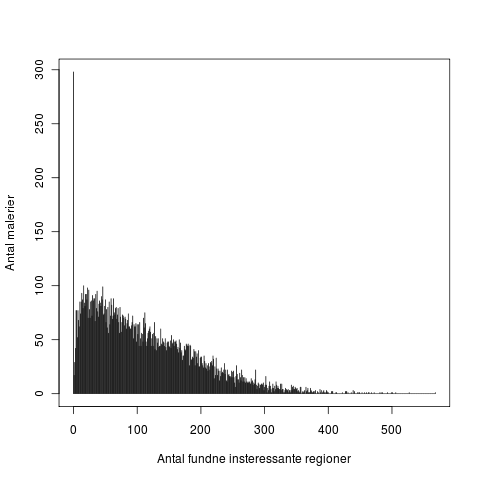
\includegraphics[width=0.49\textwidth]{afsnit/resultater/billeder/totalregions_var}
        \label{graf_total_regions_var}
    }
    \subfloat[]{
        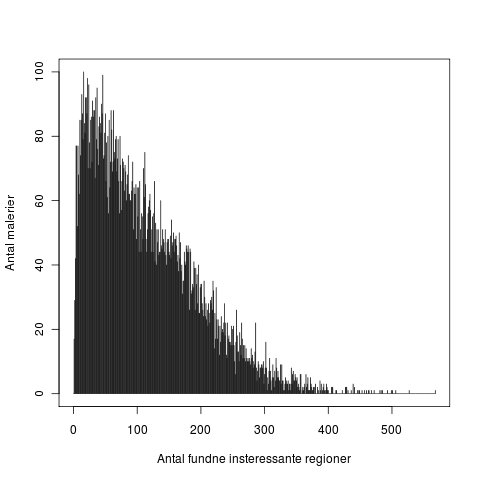
\includegraphics[width=0.49\textwidth]{afsnit/resultater/billeder/totalregions}
        \label{graf_total_regions_zoom}
    }\\
    \subfloat[]{
        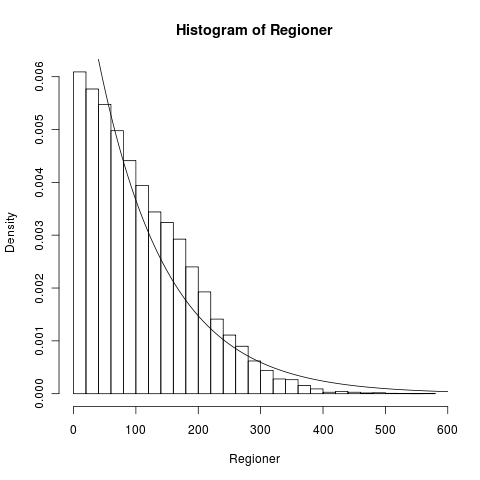
\includegraphics[width=0.62\textwidth]{afsnit/resultater/billeder/hist_totalregions}
        \label{hist_total_regions}
    }
    \caption[]{Fordelingen af fundne regioner på malerier.
    \textbf{\ref{graf_total_regions_var}:} Plot som viser hvor mange
    malerier, hvori der er fundet et vist antal interessante regioner
    over alle snit i maleriet.
    \textbf{\ref{graf_total_regions_zoom}:} Samme plot som i figur
    \ref{graf_total_regions_var}, men hvor antal malerier uden regioner
    ikke er vist.
    \textbf{\ref{hist_total_regions}:} Histogram over antal fundne
    regioner, hvor en eksponentialfordeling med $\lambda = 1/114.79$ er
    indtegnet.}
    \label{total_regions_plots}
\end{figure}

Middelværdien fortæller os at i et arbitrært maleri, kan vi forvente at
finde $115$ interessante regioner, over alle snit.  Bemærk, at en region
\emph{altid} vil ligge i fire snit og derfor meget vel kan indgå fire
gange. Endvidere skal vi huske på, at hver af disse regioner, kan være
udtrukket flere gange, på grund af den fejlbehæftede metode ti
udtrækning. Vi ser, at der er et lille antal malerier, hvori der bliver
fundet rigtig mange regioner. Det tynder dog ud omkring $380$ regioner,
hvor antallet af malerier, med flere regioner, forekommer mindre
hyppigt.

\subsection{Opsamling\label{naiv_opsamling}}
Vi har i tabel \ref{hypoteser_naiv} givet en oversigt over hvordan de
observerede værdier forholder sig til vores hypoteser. Vi vil give vores
vurdering af hvad vores data kan fortælle os om brugen af det gyldne
snit i malerier. Bemærk, at vi på ingen måde er fagfolk i
kunstforståelse, og at vores fortolkning kun er begrundet ud fra de
resultater vi har fra vores eksperiment med naiv vurdering af
interessante regioner.

\begin{table}[!h]
    \centering
    \begin{tabular}{|c|l|c|c|}
		\hline
        \textbf{Hypotese nr.} & \textbf{Beskrivelse} & \textbf{Afvist} &
        \textbf{Ikke afvist}  \\\hline\hline
        1 & Mindst én region i $GS$                     &            & \checkmark   \\\hline
        2 & Alle fire $GS$ lige meget brugt             & \checkmark &              \\\hline
        3 & $1/3$ har lærred med forholdet $1:\varphi $ & \checkmark &              \\\hline
        4 & Flest regioner i $GS$                       & \checkmark &              \\\hline
        5 & Flere regioner i $GS$ end $2/3$             &            & \checkmark   \\\hline
        6 & Flere regioner i $GS$ end i midten          & \checkmark &              \\\hline
        7 & $GS$ brugt lige meget, uanset tidsperiode   & \checkmark &              \\\hline
        8 & $GS$ brugt lige meget, uanset nationalitet  & \checkmark &              \\\hline
        9 & $2/3$ brugt som approksimation til $GS$     &            & \checkmark	\\\hline
    \end{tabular}
    \caption[]{Hypoteser i forhold til den naive kørsel. $GS$ bruges som
    forkortelse for det gyldne snit.}
    \label{hypoteser_naiv}
\end{table}

Vi kan ikke afvise hypotese 1. Vi mener, at et maleri som er komponeret
efter det gyldne snit, vil have mindst én interessant region i det
gyldne snit og vi kan derfor ikke afvise, at det gyldne snit bliver
brugt i malerkunsten.

Når vi afviser hypotese 2, betyder det, at der ikke fundet det samme
antal interessante regioner i de fire gyldne snit. Vi mener, at
\emph{hvis} det gyldne snit \emph{er} specielt æstetisk tiltalende, så
findes der en gruppering af de enkelte gyldne snit, som kunstnere
foretrækker, og at der derfor findes dele af billedet, som bliver
favoriseret af kunstnere.

Vi ser at kunstnere ikke konstruerer lærredet efter det gyldne
rektangel, da hypotese 3 afvises. Vi mener, at dette sår tvivl om,
hvorvidt det gyldne rektangel er et specielt æstetisk tiltalende format.
Hvis dette var tilfældet, ville vi forvente at flere malerier havde
dette format.

Det er vores opfattelse, at hvis kunstneren arbejder ud fra det gyldne
snit, når han komponerer et maleri, må vi forvente at finde flere
interessante regioner i det gyldne snit, end i noget andet snit i
maleriet. Vores resultater har afvist at dette kan være tilfældet, da
hypotese 4 ikke holder.

Vi har ikke afvist hypotese 5 og 9. Det betyder at antallet af
interessante regioner fundet i det gyldne snit dominerer antallet af
regioner fundet i $\frac{2}{3}$ i alle fire snit, men at der ikke er
mere end $15 \%$ afvigelse mellem disse. Dette tyder på, at når det
gyldne snit bliver brugt i et maleri, så er dette et bevidst valg fra
kunstnerens side, men noget tyder også på at snittet ved to tredjedele
bruges som approksimation til det gyldne snit. Dette er en modstrid og
vi kan derfor ikke sige noget fornuftigt om, hvorvidt det gyldne snit
bruges bevidst eller om der bruges en approksimation.

Hypotese 6 afvises, hvilket betyder at der findes flere interessante
regioner i midten af billedet, end i det gyldne snit. Dette tyder på, at
kunstneren ikke arbejder ud fra det gyldne snit, men i stedet ud fra
midten, når han komponerer et maleri.

Fordi vi afviser hypotese 7, hvor vi ser på det gennemsnitlige antal
interessante regioner i det gyldne snit pr. maleri, kan vi sige at der
er forskel på hvor mange regioner der findes i det gyldne snit
tidsperioder imellem.  Dette kan tyde på, at det gyldne snit gennem
tiden, har haft svingende popularitet. Det er spændende, som vist i
figur \ref{naiv_year}, at se, hvordan regionerne fordeler sig mht. til
de historiske milestene i det gyldne snits historie. Det tyder faktisk
på en nedgang i brugen af det gyldne snit, da Luca Pacioli udgiver sin
bog \emph{De divina propertione} i 1509\cite{markowsky1992}. Heller ikke
i 1835, hvor udtrykket \emph{det gyldne snit} bruges for første
gang\cite{markowsky1992}, ses nogen speciel ændring i brugen af det
gyldne snit.

Endelig afvises også hypotese 8. Helt konkret har vi stor afvigelse i
antallet af interessante regioner fundet i det gyldne snit mellem
nationaliteter. Vi mener at dette viser, at det gyldne har større
udbredelse og popularitet i nogle lande. Grafen i figur
\ref{naiv_nation} antyder at der i græske malerier findes mange regioner
i det gyldne snit. Vi kan dog i figur \ref{naiv_nationNrImage} se at
vores grundlag for at udtale os om netop græske malerier, er vagt, på
grund af et meget lille antal af disse malerier i datasættet. På trods
af ovenstående, tyder data dog på, at det gyldne snit er mere brugt i
visse lande.

}

% vim: set tw=72 spell spelllang=da:
